% !TEX root = ../main.tex
\appendix
\ifarxiv
\clearpage
\fi
\section{Attribute Readout}
In Tab.~\ref{tab:attrreadout} and \ref{tab:attrreadout-imageneta}, we provide
attribute readout performance with different learned representations. This is a
similar task that measures the generalizability, but it does not evaluate the
rapid learning aspect brought by few-shot learning.

\begin{table}[t]
\begin{small}
\begin{center}
\begin{tabular}{lccccccc|c}
\toprule
{\bf Mean AUC}  & {\bf RND} & {\bf PN}  & {\bf ID}  & {\bf SA}  & {\bf U}   & \gr {\bf \uftpn} & \gr {\bf \uftsa}   & {\bf SA*}  \\
\hline      
% \midrule
All (40)        &  79.18    &  88.80      & 91.29     & 90.27     & 92.80   & \gr {\bf 93.34}  & \gr {\bf 93.33}      & 94.46      \\
Train+Test (27) &  82.27    &  93.38      & 94.31     & 94.23     & 95.78   & \gr {\bf 96.53}  & \gr {\bf 96.52}      & 97.18      \\
Train (14)      &  84.40    &  96.04      & 95.34     & 96.04     & 96.43   & \gr {\bf 97.23}  & \gr {\bf 97.23}      & 97.50      \\
Test  (13)      &  79.96    &  90.52      & 93.19     & 92.63     & 95.08   & \gr {\bf 95.78}  & \gr {\bf 95.76}      & 96.84      \\
% \hline
\bottomrule
\end{tabular}
% }
\end{center}
\end{small}
% \savespacebeforesection
\caption{\textbf{Celeb-A attribute readout} performance of different
representations, measured in mean AUC. RND denotes using a randomly initialized
CNN; PN denotes ProtoNet.}
\label{tab:attrreadout}
% \savespacebeforesection
\end{table}

\section{Ablation studies}
Table~\ref{tab:l1} studies the effect of the L1 regularization. The benefit is
especially noticeable on SA* and GT, since it allows the few-shot learner to
have a sparse selection of disentangled feature dimensions.

\iflatexml
\begin{table}
\begin{small}
\begin{center}
\begin{tabular}{cllll|ll}
\toprule
                & {\bf SA}              & {\bf U}                & {\bf \uftpn}         & {\bf \uftsa}           & {\bf SA*}            & {\bf GT}            \\
\hline  
LR              & 77.4                  & 79.2                   & 82.2                 & 83.1                   & 87.1                 & 95.8                \\
\gr +L1 (1e-4)  & \gr 77.6 (+0.2)       & \gr 79.4 (+1.2)        & \gr 82.3 (+0.1)      & \gr 83.2 (+0.1)        & \gr 87.4 (+0.3)      & \gr 96.1 (+0.3)     \\
\gr +L1 (1e-3)  & \gr {\bf78.2} (+0.8)  & \gr {\bf80.2} (+1.0)   & \gr {\bf 82.4} (+0.2)& \gr {\bf83.8} (+0.7)   & \gr {\bf88.4} (+1.3) & \gr 97.1 (+1.3)     \\
\gr +L1 (1e-2)  & \gr 75.7 (\gt{--1.7}) & \gr 78.3 (\gt{--0.9})  & \gr 78.8 (\gt{--3.5})      & \gr 79.5 (\gt{--3.6})  & \gr 87.6 (+0.5)      & \gr {\bf98.2} (+2.4)\\
\bottomrule
\end{tabular}
\end{center}
\end{small}
\caption{\textbf{Effect of the L1 regularizer} on different representations for
the validation set of Celeb-A 20-shot.}
\label{tab:l1}
\end{table}
\else
\begin{table}
\begin{small}
\begin{center}
\resizebox{0.8\columnwidth}{!}{
\begin{tabular}{cllll|ll}
\toprule
                & {\bf SA}              & {\bf U}                & {\bf \uftpn}         & {\bf \uftsa}           & {\bf SA*}            & {\bf GT}            \\
\hline  
LR              & 77.4                  & 79.2                   & 82.2                 & 83.1                   & 87.1                 & 95.8                \\
\gr +L1 (1e-4)  & \gr 77.6 (+0.2)       & \gr 79.4 (+1.2)        & \gr 82.3 (+0.1)      & \gr 83.2 (+0.1)        & \gr 87.4 (+0.3)      & \gr 96.1 (+0.3)     \\
\gr +L1 (1e-3)  & \gr {\bf78.2} (+0.8)  & \gr {\bf80.2} (+1.0)   & \gr {\bf 82.4} (+0.2)& \gr {\bf83.8} (+0.7)   & \gr {\bf88.4} (+1.3) & \gr 97.1 (+1.3)     \\
\gr +L1 (1e-2)  & \gr 75.7 (\gt{--1.7}) & \gr 78.3 (\gt{--0.9})  & \gr 78.8 (\gt{--3.5})      & \gr 79.5 (\gt{--3.6})  & \gr 87.6 (+0.5)      & \gr {\bf98.2} (+2.4)\\
\bottomrule
\end{tabular}
}
\end{center}
\end{small}
\caption{\textbf{Effect of the L1 regularizer} on different representations for
the validation set of Celeb-A 20-shot.}
\label{tab:l1}
\end{table}
\fi

\begin{table}
\begin{small}
\begin{center}
\begin{tabular}{lcccc}
\toprule
{\bf Mean AUC}             & {\bf SA}  & {\bf SA*}  & {\bf U}   & {\bf UFTA}   \\
\hline

\hline
 All (25 attributes)        & 72.01 & 73.02 & 81.08 & \textbf{82.49} \\
 Train+Test (21 attributes) & 73.43 & 78.98 & 80.14 & \textbf{82.37} \\
 Train (11 attributes)      & 72.69 & 75.86 & 80.63 & \textbf{82.43} \\
 Test (10 attributes)       & 72.01 & 74.98 & 81.08 & \textbf{83.30} \\
\hline
\end{tabular}
\end{center}
% \fi
\end{small}
% \savespacebeforesection
\caption{ImageNet-with-Attributes attribute readout binary prediction
performance of different representations, measured in mean AUC. }
\label{tab:attrreadout-imageneta}
% \savespacebeforesection
\end{table}

\section{Additional heatmap visualization}

We provide additional visualization results in
Figure~\ref{fig:additional_combo}, \ref{fig:celeb-a-additional}, and
\ref{fig:zappos-additional}, and we plot the heat map to visualize the LR
classifier weights. Figure~\ref{fig:additional_combo} includes SA*, U, and UFTE
which are omitted in the main paper due to space limitations.
Figure~\ref{fig:celeb-a-additional} and \ref{fig:zappos-additional} visualize
more information including both support and query examples in the episode, and
some of the episodes are challenging to solve given just a few examples.

\begin{figure*}[t]
\centering
\iflatexml
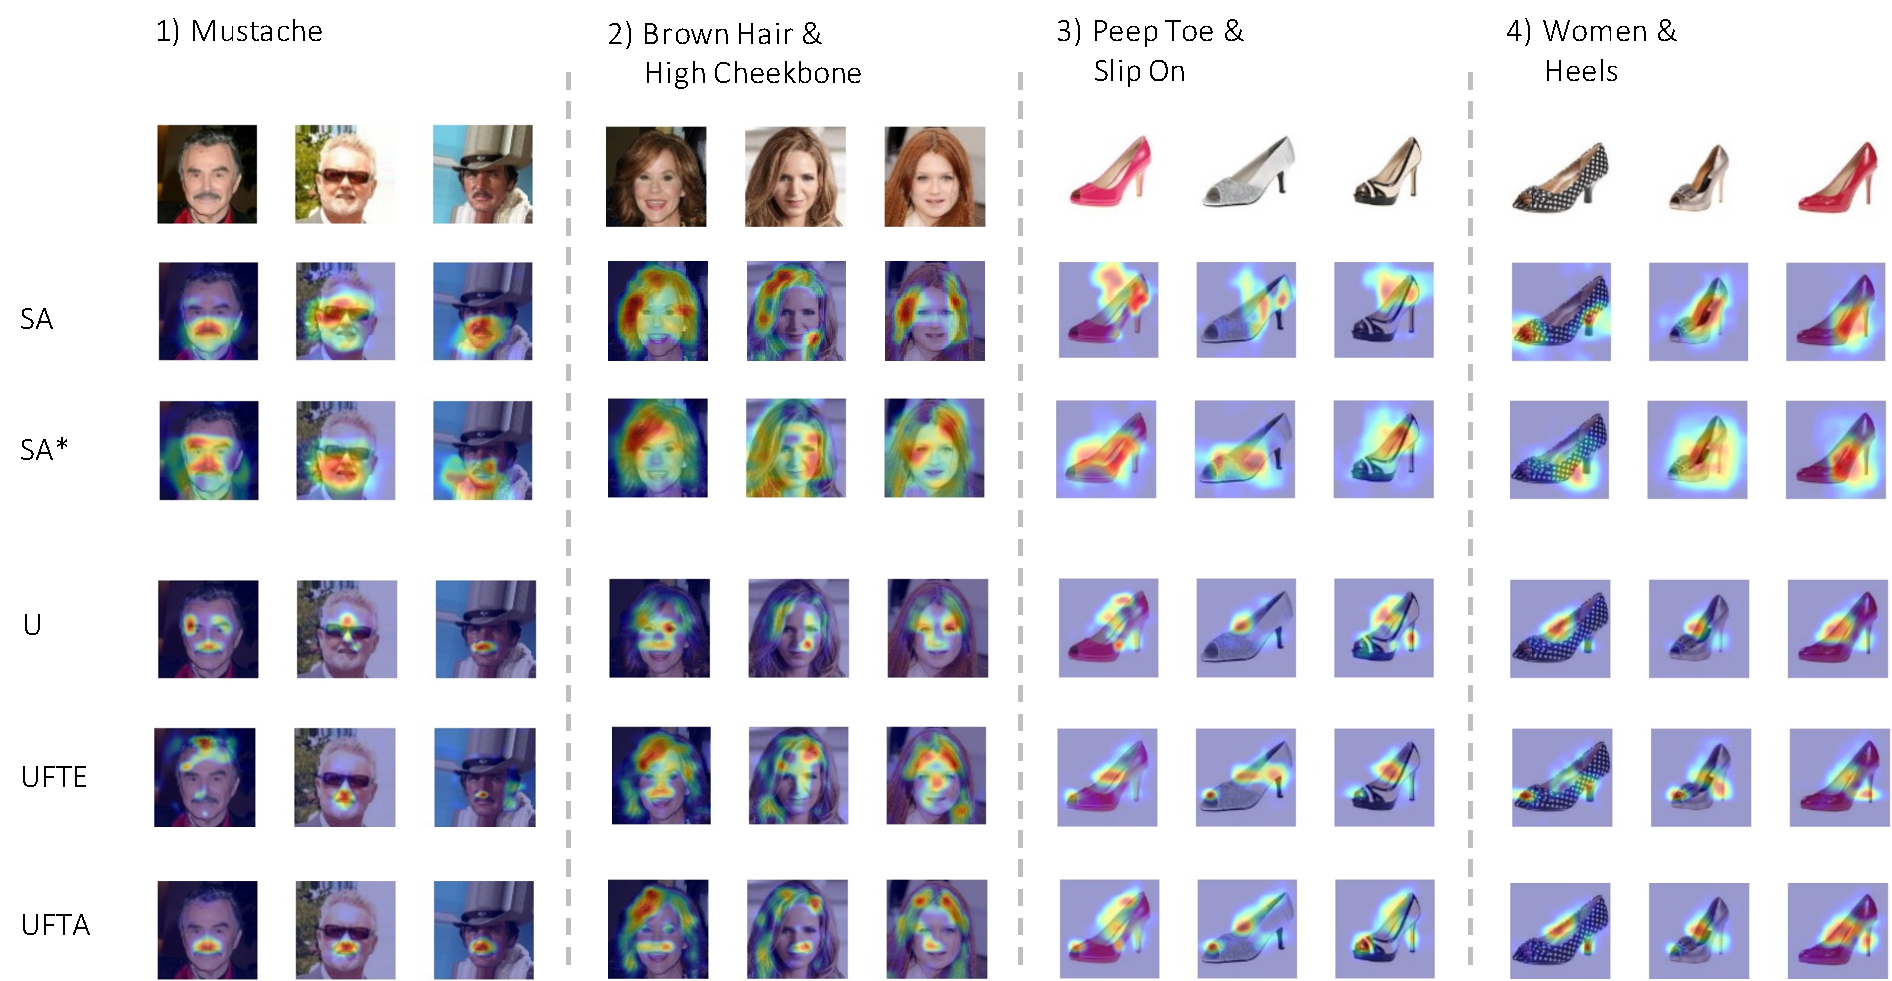
\includegraphics[width=6\linewidth]{figures/vis_cam_iccv_supp.png}
\else
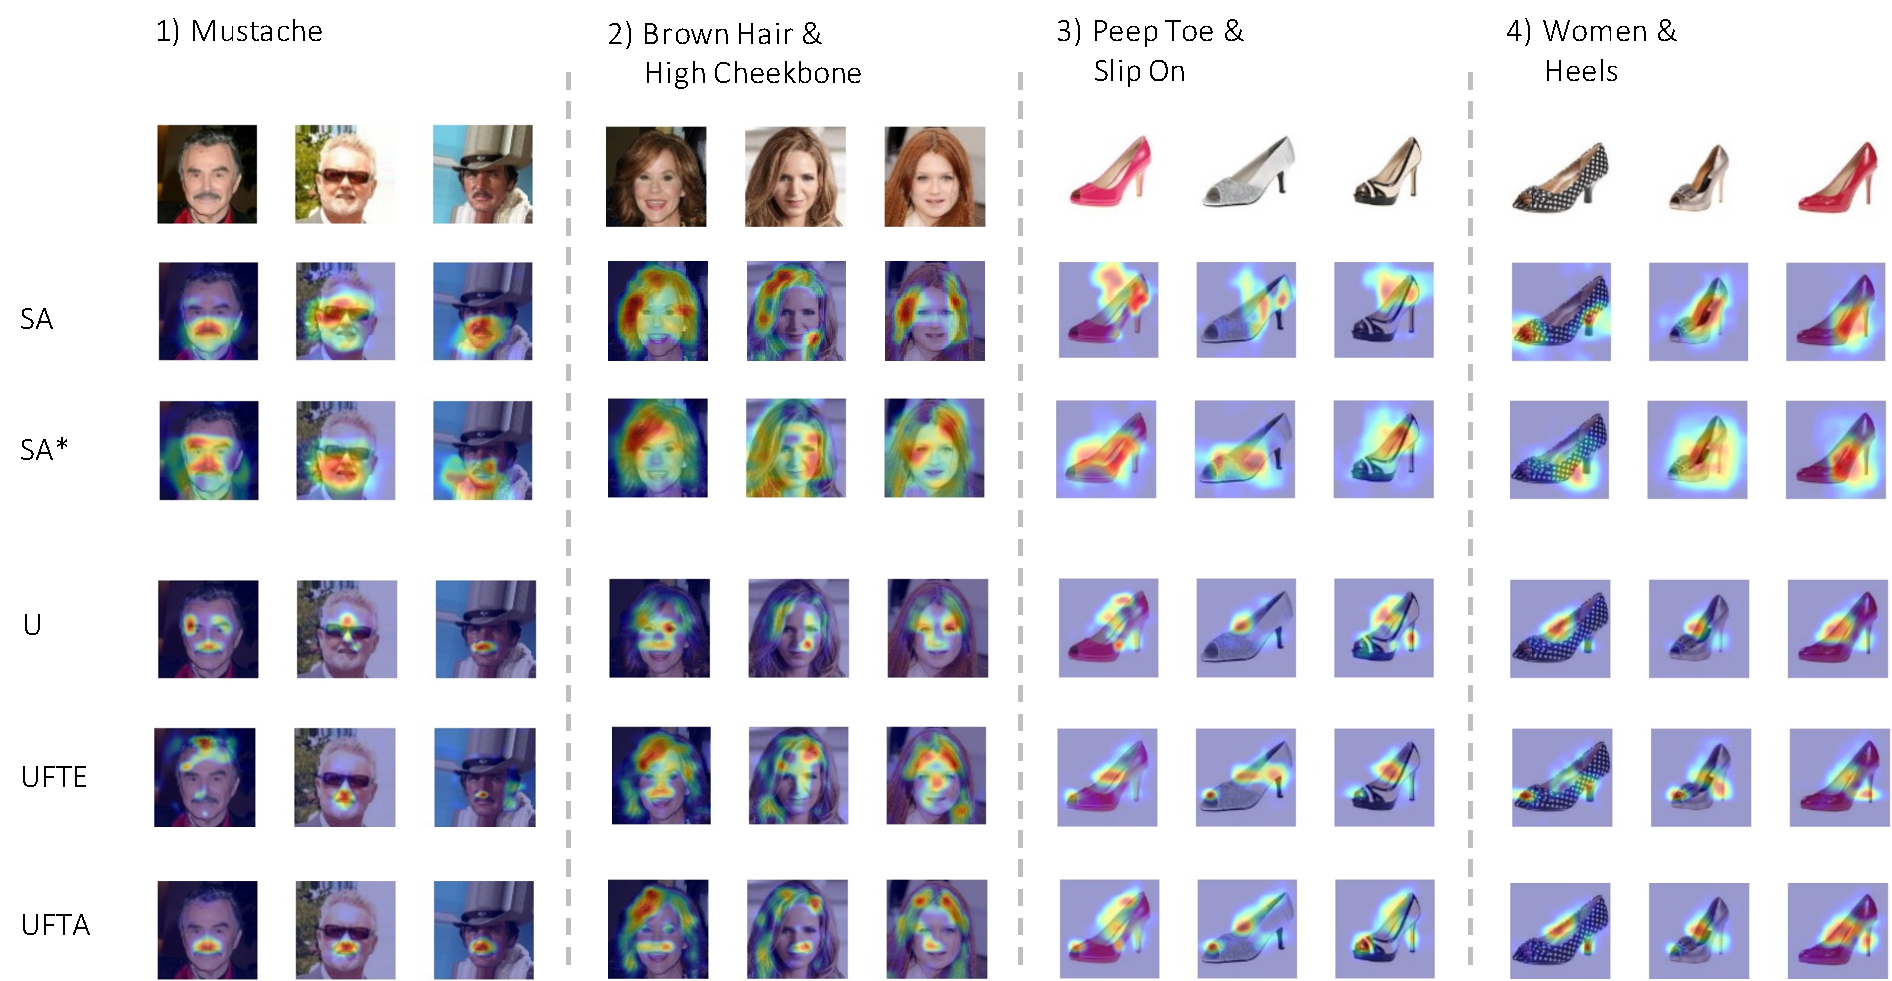
\includegraphics[width=0.9\linewidth]{figures/vis_cam_iccv_supp.pdf}
\fi
\caption{Additional visualization results, on 20-shot episodes, including more
methods for comparison.}
\label{fig:additional_combo}
\end{figure*}

\begin{figure*}[t]
\centering
\iflatexml
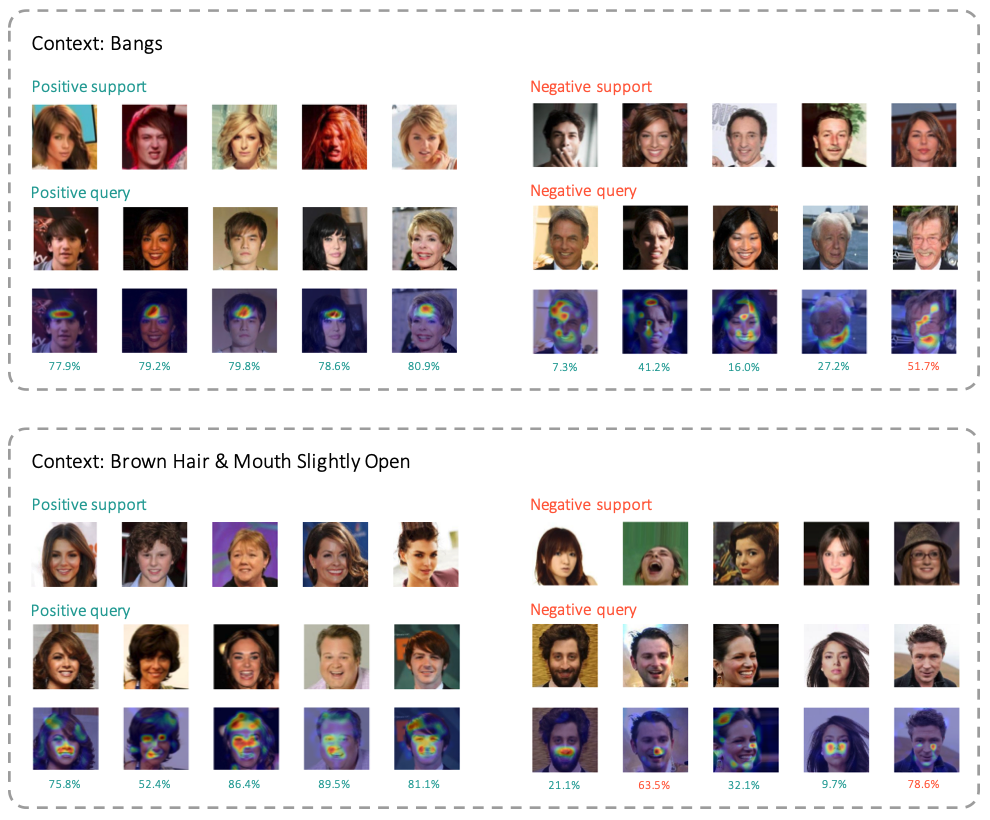
\includegraphics[width=6\linewidth]{figures/additional_viz_celeb.png}
\else
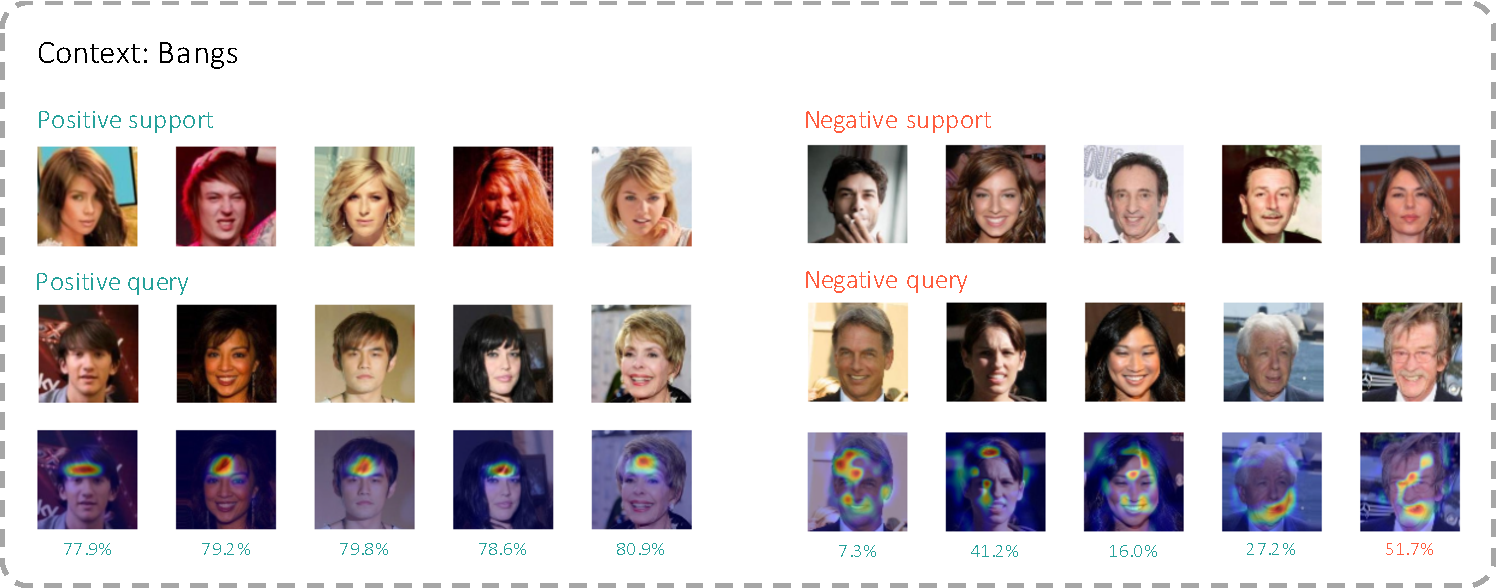
\includegraphics[width=0.9\linewidth]{figures/additional_viz_celeb_1.pdf}\\
\quad \\
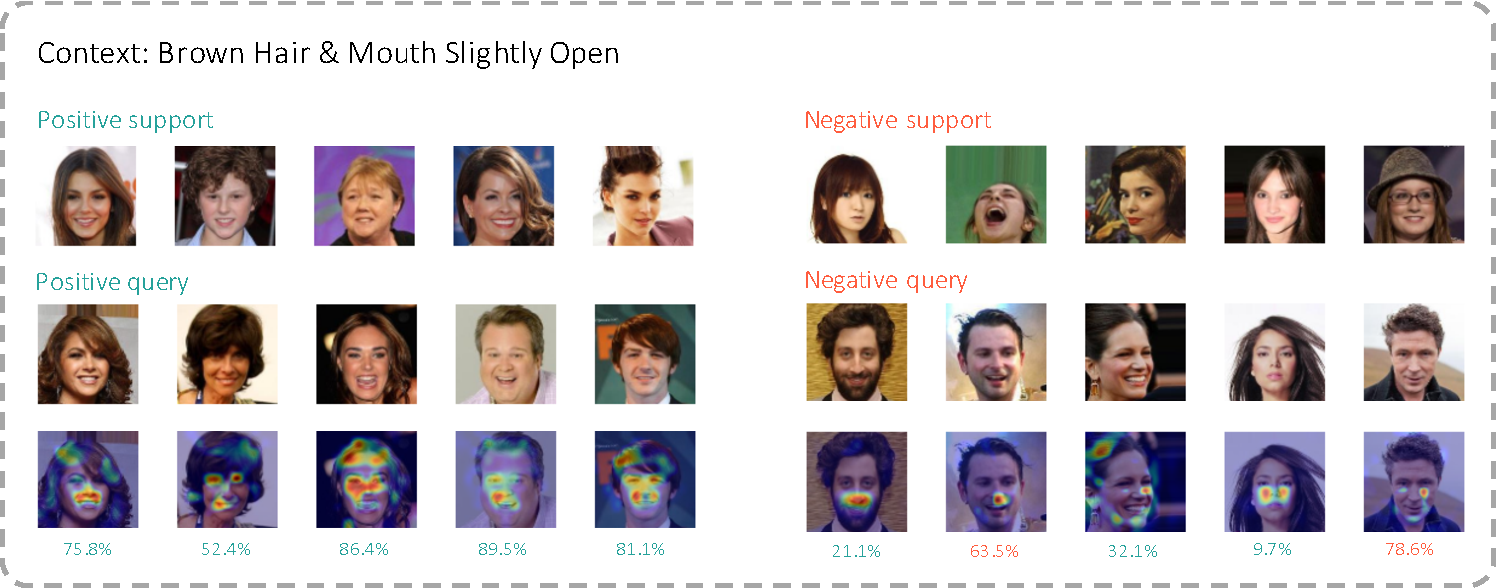
\includegraphics[width=0.9\linewidth]{figures/additional_viz_celeb_2.pdf}
\fi
\caption{\textbf{Visualization of Celeb-A 20-shot LR classifiers using CAM on
top of UFTA representations.} Context attributes that define the episode are
shown above. Classifier sigmoid confidence scores are shown at the bottom. Red
numbers denote wrong classification and green denote correct. }
\label{fig:celeb-a-additional}
\end{figure*}
\begin{figure*}[t]
\centering
\iflatexml
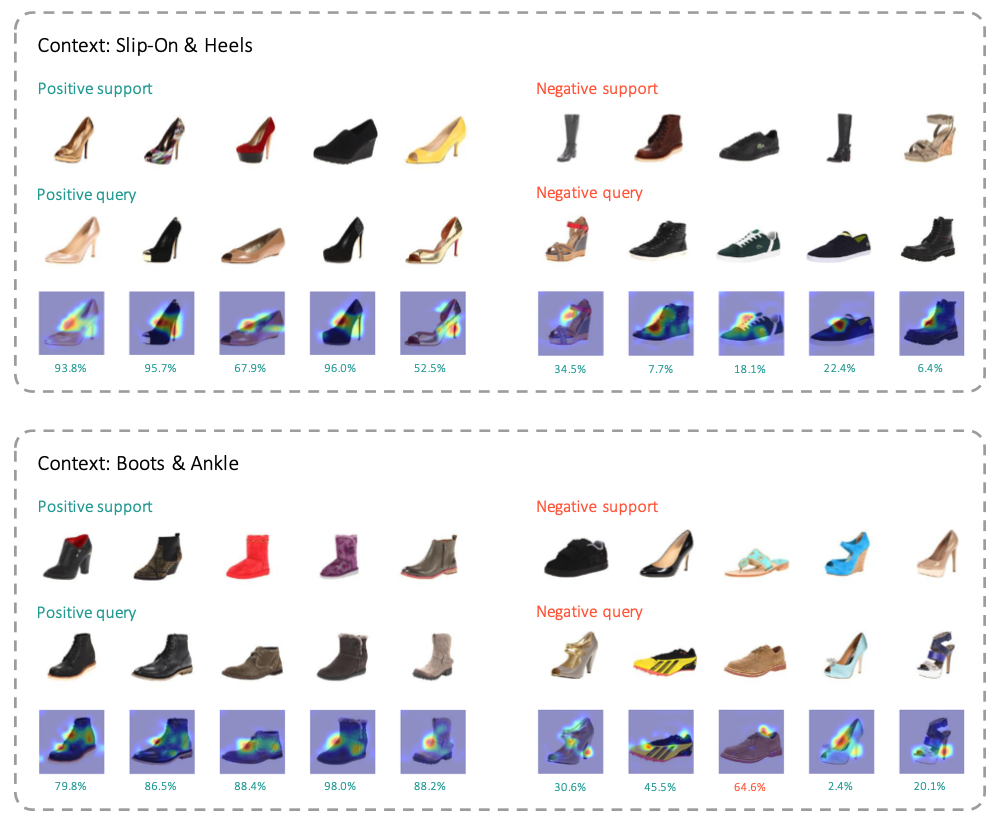
\includegraphics[width=6\linewidth]{figures/additional_viz_zappos.png}
\else
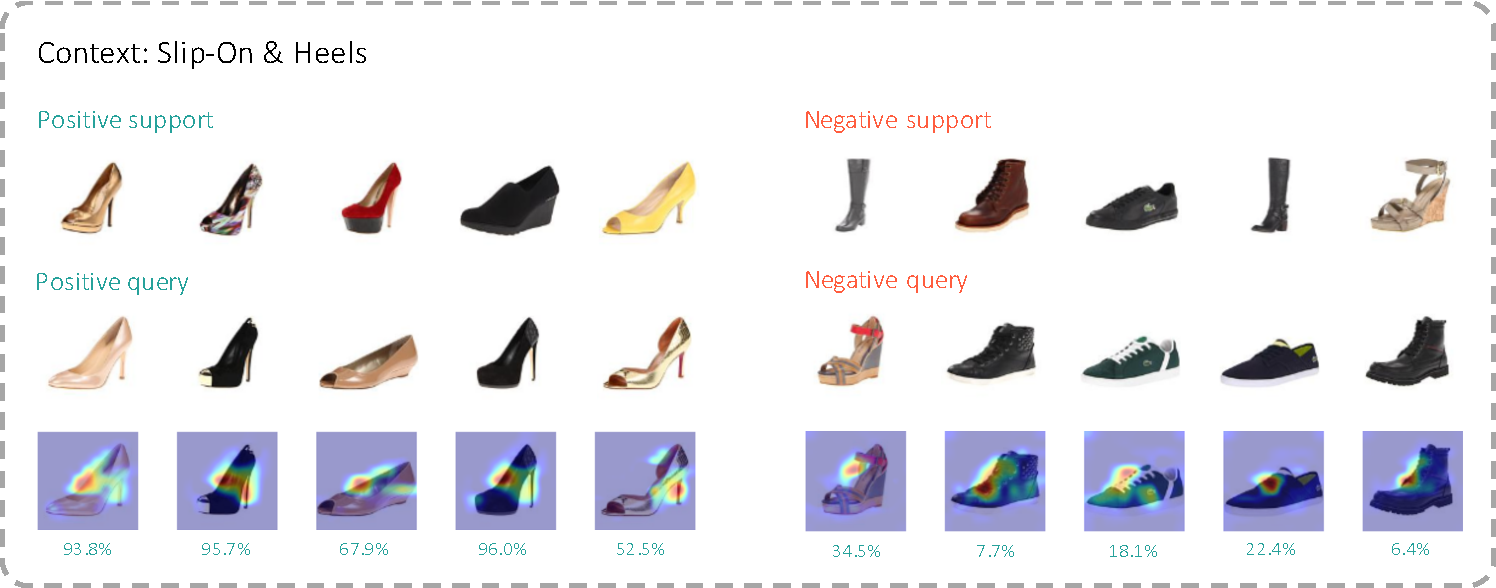
\includegraphics[width=0.9\linewidth]{figures/additional_viz_zappos_1.pdf}\\
\quad \\
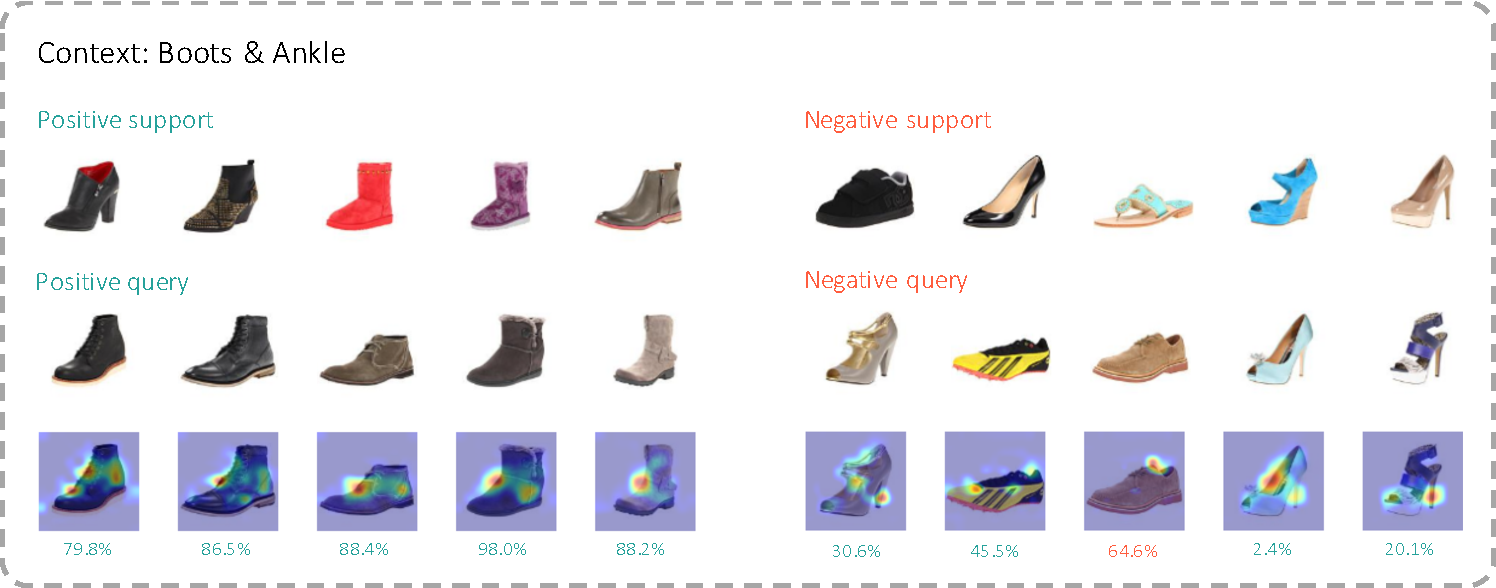
\includegraphics[width=0.9\linewidth]{figures/additional_viz_zappos_2.pdf}
\fi
\caption{\textbf{Visualization of Zappos-50K 20-shot LR classifiers using CAM
on top of UFTA representations.} Context attributes that define the episode are
shown above. Classifier sigmoid confidence scores are shown at the bottom. Red
numbers denote wrong classification and green denote correct. }
\label{fig:zappos-additional}
\end{figure*}

% !TEX root = ../iccv2021_supp.tex
\begin{table*}[t]
\centering
% \vspace{-0.5in}
\begin{center}
\begin{small}
% \resizebox{0.98\textwidth}{!}{
\begin{tabular}{ccccc}
% \toprule
\hline
\mr{4}{\textbf{Train}} &
5\_o\_Clock\_Shadow & 
Black\_Hair & 
Blond\_Hair & 
Chubby\\
& 
Double\_Chin & 
Eyeglasses & 
Goatee & 
Gray\_Hair\\
& 
Male & 
No\_Beard & 
Pale\_Skin & 
Receding\_Hairline\\
& 
Rosy\_Cheeks & 
Smiling &  &  \\
% \midrule
\hline
\mr{4}{\textbf{Val/Test}} &
Bald & 
Bangs & 
Brown\_Hair & 
Heavy\_Makeup\\
& 
High\_Cheekbones & 
Mouth\_Slightly\_Open & 
Mustache & 
Narrow\_Eyes\\
& 
Sideburns & 
Wearing\_Earrings & 
Wearing\_Hat & 
Wearing\_Lipstick\\
& 
Wearing\_Necktie & &  &  \\
% \bottomrule
\hline
\end{tabular}
% }
\end{small}
\end{center}
\caption{Attribute Splits for Celeb-A}
\label{tab:celebasplit}
\end{table*}

\section{Attribute splits of Celeb-A}
\label{app:split}
We include the attribute split for Celeb-A in Table~\ref{tab:celebasplit}. There are 14 attributes
in training and 13 attributes in val/test. We discarded the rest of the 13 attributes in the
original datasets since they are either hard to classify with the oracle classifier (e.g. big lips, oval face) or simply ambiguous (e.g. young, attractive).
% !TEX root = ../cvpr2021/supp.tex
\begin{table*}[t]
\centering
% \vspace{-0.5in}
\begin{center}
\begin{small}
\resizebox{0.98\textwidth}{!}{
\begin{tabular}{ccccc}
% \toprule
\hline
\mr{10}{\textbf{Train}} &
Category-Shoes &
Category-Sandals &
SubCategory-Oxfords &
SubCategory-Heel \\
&
SubCategory-Boot &
SubCategory-Slipper Flats & SubCategory-Short heel& SubCategory-Flats \\
&
SubCategory-Slipper Heels & SubCategory-Athletic &
SubCategory-Knee High &
SubCategory-Crib Shoes \\
&
SubCategory-Over the Knee &
HeelHeight-High heel &
Closure-Pull-on &
Closure-Ankle Strap \\
&
Closure-Zipper & 
Closure-Elastic Gore &
Closure-Sling Back &
Closure-Toggle \\
&
Closure-Snap &
Closure-T-Strap &
Closure-Spat Strap &
Gender-Men \\ 
&
Gender-Boys & 
Material-Rubber &
Material-Wool & 
Material-Silk \\
&
Material-Aluminum &
Material-Plastic &
Toestyle-Capped Toe &
Toestyle-Square Toe \\
&
Toestyle-Snub Toe &
Toestyle-Bicycle Toe &
Toestyle-Open Toe &
Toestyle-Pointed Toe \\
&
Toestyle-Almond &
Toestyle-Apron Toe &
Toestyle-Snip Toe &
Toestyle-Medallion\\
\hline

\mr{10}{\textbf{Val/Test}} &
Category-Boots & 
Category-Slippers & 
SubCategory-Mid-Calf & 
SubCategory-Ankle \\
&
SubCategory-Loafers & 
SubCategory-Boat Shoes & 
SubCategory-Clogs and Mules &
SubCategory-Sneakers and Athletic Shoes \\
&
SubCategory-Heels & 
SubCategory-Prewalker &
SubCategory-Prewalker Boots & SubCategory-Firstwalker \\
&
HeelHeight-Short heel &
Closure-Lace up & 
Closure-Buckle & 
Closure-Hook and Loop \\
&
Closure-Slip-On &
Closure-Ankle Wrap &
Closure-Bungee &
Closure-Adjustable \\
&
Closure-Button Loop &
Closure-Monk Strap &
Closure-Belt &
Gender-Women \\
&
Gender-Girls &
Material-Suede &
Material-Snakeskin &
Material-Corduroy \\
&
Material-Horse Hair &
Material-Stingray &
Toestyle-Round Toe &
Toestyle-Closed Toe \\
&
Toestyle-Moc Toe &
Toestyle-Wingtip &
Toestyle-Center Seam &
Toestyle-Algonquin \\
&
Toestyle-Bump Toe &
Toestyle-Wide Toe Box &
Toestyle-Peep Toe & \\
\hline
\end{tabular}
}
\end{small}
\end{center}
% \vspace{-0.2in}
\caption{Attribute splits for Zappos-50K}
\label{tab:zappossplit}
\end{table*}

% \textbf{Training attributes:} Category-Shoes, Category-Sandals, SubCategory-Oxfords, SubCategory-Heel, SubCategory-Boot, SubCategory-Slipper Flats, SubCategory-Short heel, SubCategory-Flats, SubCategory-Slipper Heels, SubCategory-Athletic, SubCategory-Knee High, SubCategory-Crib Shoes, SubCategory-Over the Knee, HeelHeight-High heel, Closure-Pull-on, Closure-Ankle Strap, Closure-Zipper, Closure-Elastic Gore, Closure-Sling Back, Closure-Toggle, Closure-Snap, Closure-T-Strap, Closure-Spat Strap, Gender-Men, Gender-Boys, Material-Rubber, Material-Wool, Material-Silk, Material-Aluminum, Material-Plastic, Toestyle-Capped Toe, Toestyle-Square Toe, Toestyle-Snub Toe, Toestyle-Bicycle Toe, Toestyle-Open Toe, Toestyle-Pointed Toe, Toestyle-Almond, Toestyle-Apron Toe, Toestyle-Snip Toe, Toestyle-Medallion.

% \textbf{Held-out attributes:} Category-Boots, Category-Slippers, SubCategory-Mid-Calf, SubCategory-Ankle, SubCategory-Loafers, SubCategory-Boat Shoes, SubCategory-Clogs and Mules, SubCategory-Sneakers and Athletic Shoes, SubCategory-Heels, SubCategory-Prewalker, SubCategory-Prewalker Boots, SubCategory-Firstwalker, HeelHeight-Short heel, Closure-Lace up, Closure-Buckle, Closure-Hook and Loop, Closure-Slip-On, Closure-Ankle Wrap, Closure-Bungee, Closure-Adjustable, Closure-Button Loop, Closure-Monk Strap, Closure-Belt, Gender-Women, Gender-Girls, Material-Suede, Material-Snakeskin, Material-Corduroy, Material-Horse Hair, Material-Stingray, Toestyle-Round Toe, Toestyle-Closed Toe, Toestyle-Moc Toe, Toestyle-Wingtip, Toestyle-Center Seam, Toestyle-Algonquin, Toestyle-Bump Toe, Toestyle-Wide Toe Box, Toestyle-Peep Toe.

\section{Attribute splits of Zappos-50K}
% \subsection{Description of the data}
The Zappos-50K dataset annotates images with different values relating to the following aspects of shoes: `Category', `Subcategory', `HeelHeight', `Insole', `Closure', `Gender', `Material' and `Toestyle'.

We discarded the `Insole' values, since those refer to the inside part of the shoe which isn't visible in the images. We also discarded some `Material' values that we deemed hard to recognize visually. We also modified the values of `HeelHeight' which originally was different ranges of cm of the height of the heel of each shoe. Instead, we divided those values into only two groups: `short heel' and `high heel', to avoid having to perform very fine-grained heel height recognition which we deemed was too difficult.

These modifications leave us with a total of 79 values (across all higher-level categories). Not all images are tagged with a value from each category, while some are even tagged with more than one value from the same category (e.g. two different materials used in different parts of the shoe). We split these values into 40 `training attributes' and 39 `val/test attributes'. %As mentioned in the main paper, the training attributes are used to construct training episodes (when performing episodic training), or to define the classification layer (in the case of the SA and UFT models). The `val/test attributes', on the other hand, are used to construct our flexible evaluation episodes. For example, a particular training episode might define its positive class as the conjunction: `Category=Sandals and Material=Plastic' and a test episode might define its positive class as the conjunction: `Category=Boots and Closure=Buckle'.

% \subsection{List of attributes per split}
We include the complete list of attributes in Table~\ref{tab:zappossplit}. The format we use is `X-Y' where X stands for the category (e.g. `Material') and Y stands for the value of that category (e.g. `Wool'). We do this to avoid ambiguity, since it may happen that different categories have some value names in common, e.g. `Short Heel' is a value of both `SubCategory' and `HeelHeight'.

% !TEX root = ../arxiv/main.tex
% train_strs
% ['pink', 'spotted', 'wet', 'blue', 'shiny', 'rough', 'striped', 'white', 'metallic', 'wooden', 'gray']
% val_strs
% ['brown', 'green', 'violet', 'red', 'orange', 'yellow', 'furry', 'black', 'vegetation', 'smooth']

\begin{table*}[t]
\centering
% \vspace{-0.5in}
\begin{center}
\begin{small}
% \resizebox{0.98\textwidth}{!}{
\begin{tabular}{ccccc}
% \toprule
\hline
\mr{4}{\textbf{Train}} &
pink & 
spotted & 
wet & 
blue\\
& 
shiny & 
rough & 
striped & 
white\\
& 
metallic & 
wooden & 
gray & 
\\
% \midrule
\hline
\mr{4}{\textbf{Val/Test}} &
brown & 
green & 
violet & 
red\\
& 
orange & 
yellow & 
furry & 
black\\
& 
vegetation & 
smooth & 
 & 
\\
% \bottomrule
\hline
\end{tabular}
% }
\end{small}
\caption{Attribute Splits for ImageNet-with-Attributes}
\label{tab:imageneta-split}
\end{center}
\end{table*}

\section{Attribute splits of ImageNet-with-Attributes}
\label{app:imageneta-split}
We include the attribute split for ImageNet-with-Attributes in Table~\ref{tab:imageneta-split}.
There are 11 attributes in training and 10 attributes in val/test. We discarded the rest of the 4
attributes in the ``shape'' category (long, round, rectangular and square), since they are difficult to predict from the images.
% !TEX root = ../arxiv.tex
\section{Few-Shot Attribute Learning Toy Problem}
\label{app:toy_problem}

In this section, we present a toy problem that illustrates the challenges introduced by the FSAL setting and the failures of existing approaches on this task. This simple problem
captures the core elements of our FSAL tasks, including ambiguity, introducing novel attributes at test time, and the role of learning good representations. The primary limitation of this
model is the fact that it is fully linear and the attribute values are independent---in a more
realistic FSAL task recovering a good representation from the data is significantly more
challenging, and the data points will have a more complex relationship with the attributes as in our
benchmark datasets.

\paragraph{Problem setup} We define a FSAL problem where the data points $\bx
\in \bbR^{m}$ are generated from binary attribute strings, $\bz \in \{0, 1\}^d$, with $\bx = A \bz +
\bzeta$ for some matrix $A \in \bbR^{m \times d}$ with full column rank and noise source $\bzeta$.
Thus, each data point $\bx$ is a sum of columns of $A$ with some additive noise.

In each episode, examples are labelled as positive when two designated entries of the attribute strings are both 1-valued,
and negative otherwise. For the training episodes, the labels depend only on the first $d_1 < d$
entries of $\bz$. At test time, the labels depend on the remaining $d -d_1$ attributes. The training and test
episodes are generated by choosing two of the attributes in the respective sets. Then $k$ data points are sampled with positive labels (the two attributes are 1-valued) and $k$ with negative labels (at least one of the attributes is
0-valued).

\begin{figure}
    \iflatexml
        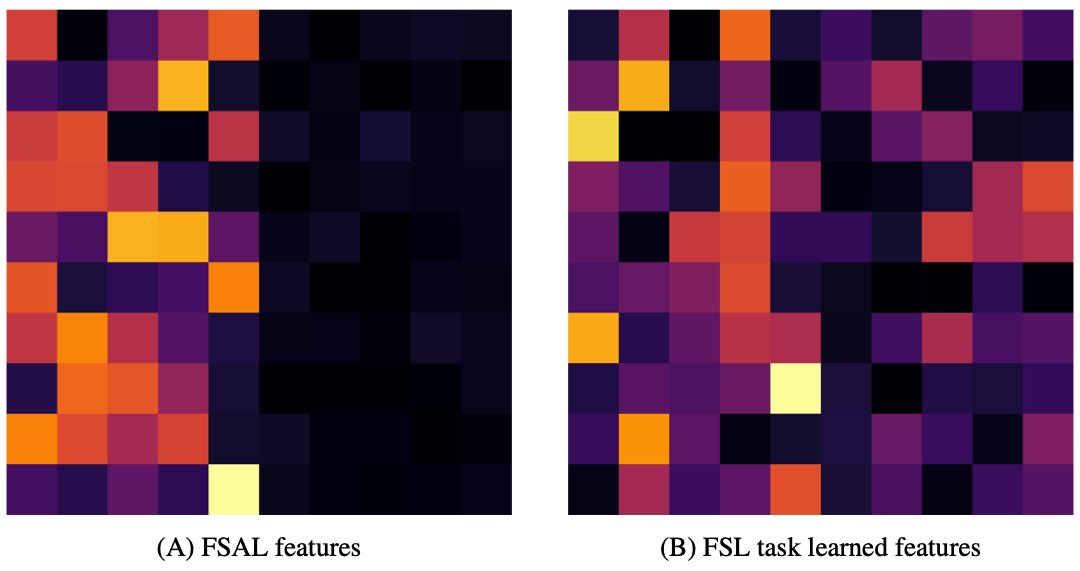
\includegraphics[width=6\linewidth]{figures/WA_abs_inferno.png}
    \else
    \begin{minipage}{0.48\linewidth}
    \centering
    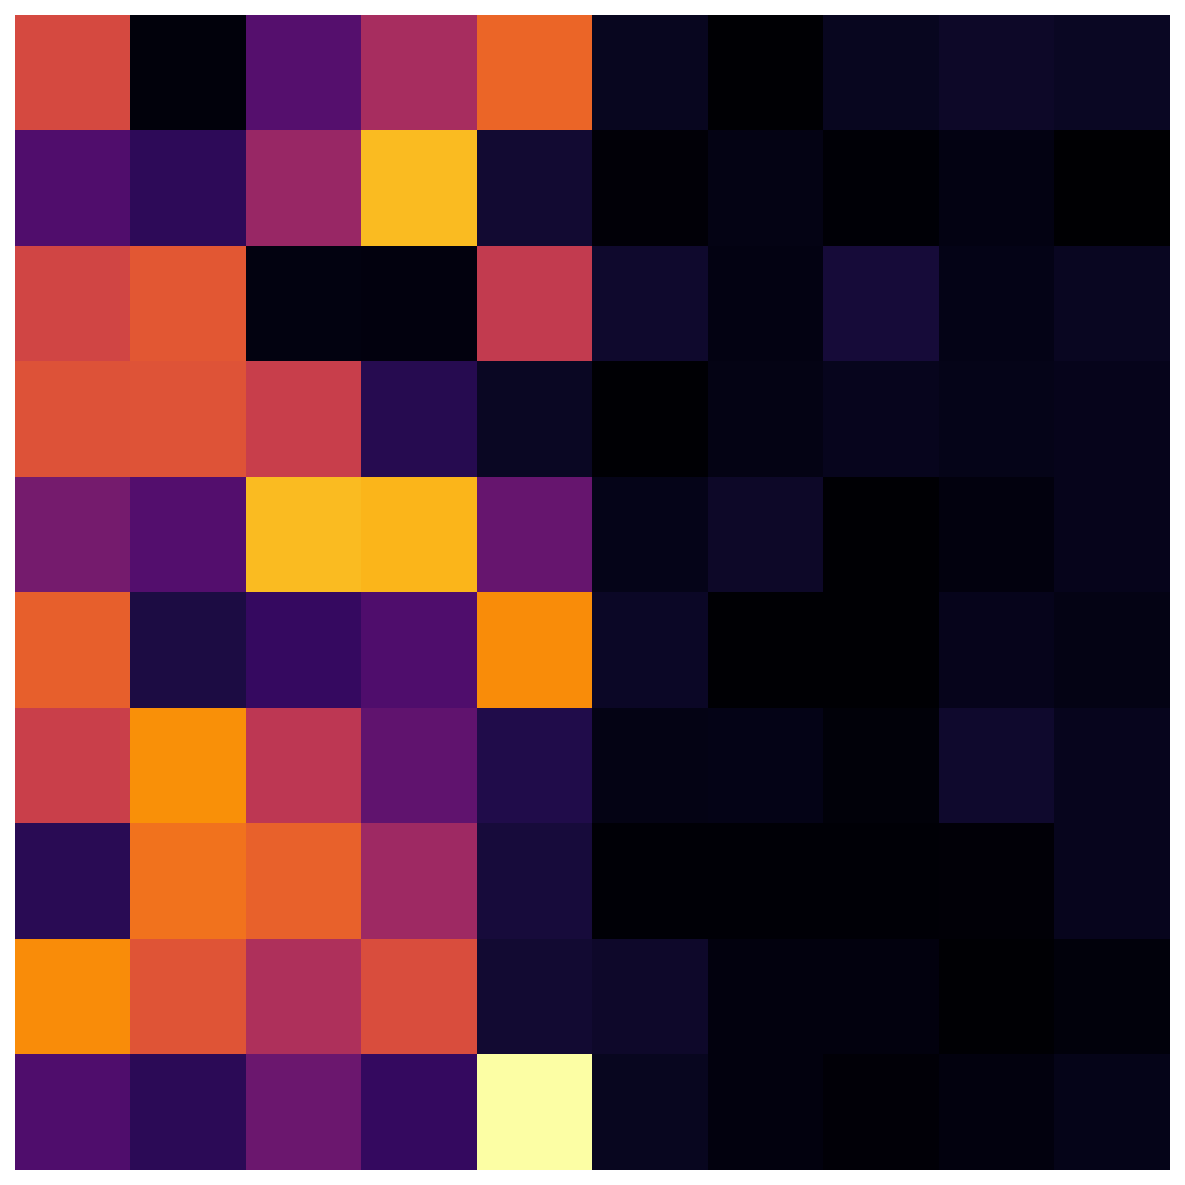
\includegraphics[width=\linewidth]{figures/WA_abs_flexible_inferno.pdf}\\
    (A) FSAL features
    \end{minipage}\hfill%
    \begin{minipage}{0.48\linewidth}
    \centering
    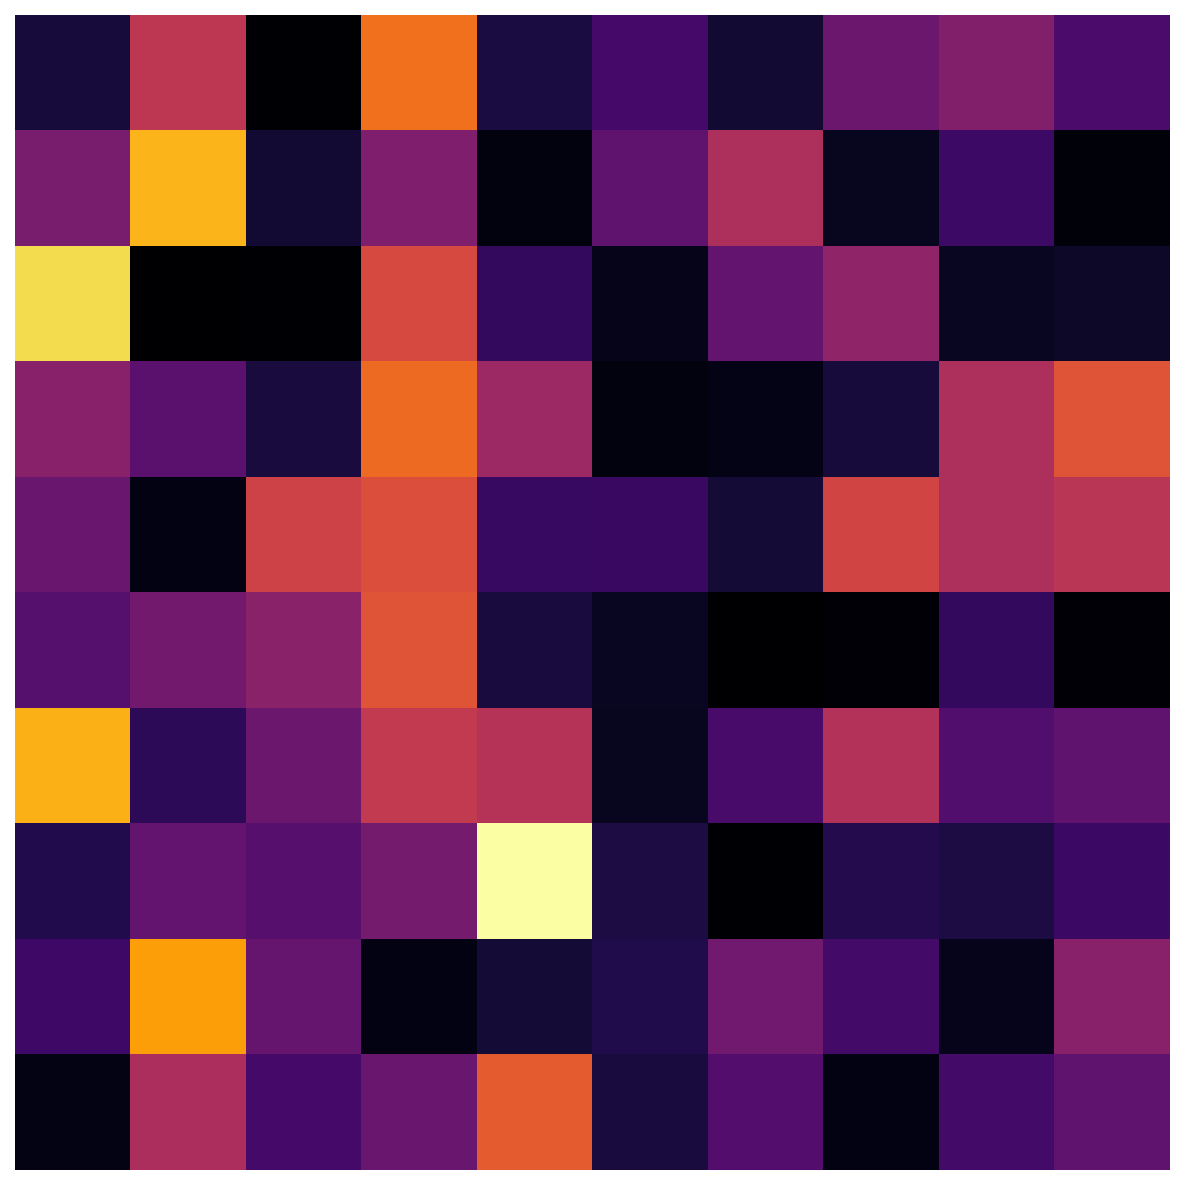
\includegraphics[width=\linewidth]{figures/WA_abs_standard_inferno.pdf}\\
    (B) FSL task learned features
    \end{minipage}
    \fi
    \caption{Projecting data features into prototypical network embedding space ($WA$) for the
    linear toy problem. Values closer to zero are darker in colour. On the FSAL task, the model
    destroys information from the test attributes to remove ambiguity at training time.}
    \label{fig:toy_problem_weights}
\end{figure}
\paragraph{Linear prototypical network} Now, consider training a prototypical network on this data
with a linear embedding network, $g(\bx)~=~W\bx$. Within each episode, the prototypical network
computes the prototypes for the positive and negative examples,
\[
\bc_{j} = \frac{1}{k}\sum_{\bx_i \in S_j} g(\bx_i)
= \frac{1}{k}\sum_{\bx_i \in S_j} \sum_{l=1}^{d}z_{il}W\ba_{l},\textrm{ for }j \in \{0, 1\},
\]
where $S_j$ is the set of data points in the episode with label $j$, and $\ba_{l}$ is the
$l^{\text{th}}$ column of the matrix $A$. Further, the prototypical network likelihood is given
by,
\[p(y=0|\bx) = \frac{\exp\left\{-\Vert W\bx - \bc_0 \Vert^2_2\right\}}{\exp\left\{-\Vert W\bx -
\bc_0 \Vert^2_2\right\} + \exp\left\{-\Vert W\bx - \bc_1 \Vert^2_2\right\}}.\] The goal of the
prototypical network is thus to learn weights $W$ that lead to small distances between data points
in the same class and large distances otherwise. In the FSAL tasks, there is
an additional challenge in that class boundaries shift between episodes. The context (the choice of attribute entries) defining the
boundary is unknown and must be inferred from the episode. However, with few shots (small $k$) there
is ambiguity in the correct context --- with a high probability that several possible contexts
provide valid explanations for the observed data.

\paragraph{Fitting the prototypical network}
Notice that under our generative model, with $\bx = W\bz + \bzeta$ and for $j \in \{0, 1\}$ we have,
\begin{align*}
W\bx - \bc_j =\ & W A (\bz - \frac{1}{k}\sum_{\bz_i \in S_j} \bz_i) + %\\ &
\frac{1}{k}\sum_{i}W\bzeta_i +
W\bzeta.
\end{align*}
% \]
Notice that if $\rvv_j(\bz) = A (\bz - \frac{1}{k}\sum_{\bz_i \in S_j} \bz_i)~\in~\textrm{Ker}(W)$,
the kernel of $W$, then the entire first term is zero. Further, if $\bz \in S_j$ (the same class as
the prototype) then there is no contribution from the positive attribute features in this term.
Otherwise, this term is guaranteed to have some contribution from the positive attribute features.

Therefore, if $W$ projects to the linear space spanned by the positive attribute features then
$W\rvv_j(\bz)$ is zero when $\bz \in S_j$ and non-zero otherwise. This means that the model will be
able to solve the episode without contextual ambiguity. Then the optimal weights are those that
project to the set of features used in the training set---destroying all information about the test
attributes which would otherwise introduce ambiguity.

We observed this effect empirically in Figure~\ref{fig:toy_problem_weights}, where we have plotted
the matrix $\mathrm{abs}(WA)$. Each column of these plots represents a column of $A$ mapped to the
prototypical network's embedding space. The first 5 columns correspond to attributes used at
training time, and the remaining 5 to those used at test time.

In the FSAL task described above, as our analysis suggests, the learned prototypical feature
weights project out the features used at test time (the last 5 columns). As a result, the model
achieved 100\% training accuracy but only 51\% test accuracy (chance is 50\%).

We also compared against an equivalent problem set up that resembles the standard few-shot learning setting. In the FSL problem, the binary attribute strings may have only a single non-zero entry and each episode is a binary classification problem where the learner must distinguish between two classes. Now the vector $\bz$ is a one-hot encoding and the comparison to the prototypes occurs only over a single feature column of $A$, thus there is no benefit to projecting out the test features. As expected, the model we learned (Figure~\ref{fig:toy_problem_weights} B) is not forced to throw away test-time information and achieves 100\% training accuracy and 99\% test accuracy.

\paragraph{Settings for Figure~\ref{fig:toy_problem_weights}} We use 10 attributes, 5 of which are
used for training and 5 for testing. We use a uniformly random sampled $A\in\bbR^{30\times10}$ and
the prototypical network learns $W\in\bbR^{10\times30}$. We use additive Gaussian noise when
sampling data points with a standard deviation of 0.1. The models are trained with the Adam
optimizer using default settings over a total of 30000 random episodes, and evaluated on an
additional 1000 test episodes. We used $k=20$ to produce these plots, but found that the result was
consistent over different shot counts.

